\section{Beamline}

The CLAS12 beamline is made up of several pieces, each discussed below. The positioning and composition of the beamline
depends on the run configuration, that can be:

\begin{itemize}
	\item FTOn: Forward Tagger present and operational. The Moller shield starts at z=877 mm from the target center to.
	\item FTOff: FT is present but not operational. The FT tracker is replaced by shielding.
                 The Moller shield starts at z=430 mm from the target center, and additional shielding is present to connect it to the FT.
\end{itemize}


\begin{figure}
	\centering
	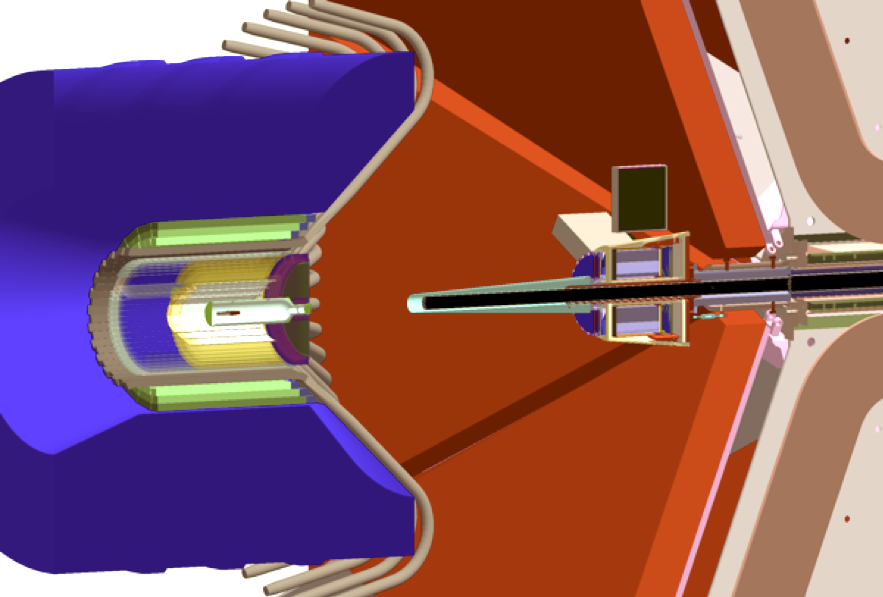
\includegraphics[width=0.98\columnwidth,keepaspectratio]{img/ftOnGeometry.png}
	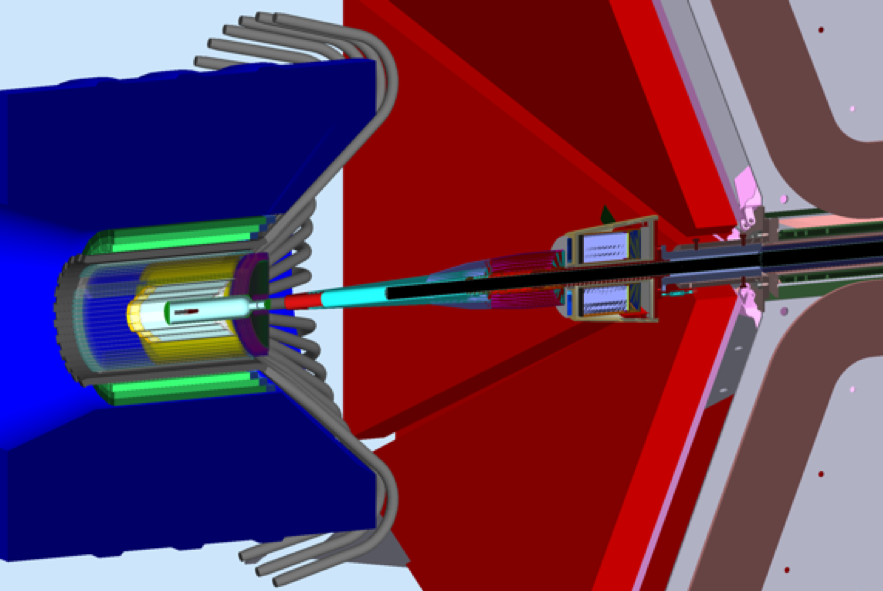
\includegraphics[width=0.98\columnwidth,keepaspectratio]{img/ftOffGeometry.png}
   \caption{The two possible CLAS12 configurations. Top: FTOn. To clear its acceptance at forward angles ($2.50-4.50$ degrees)
            the Moller shield (cyan color) is attached to the FT tracker, starting at $z=877$ mm from the target.
            Bottom: FToff; the FT is present but not operational. The FT tracker is replaced with a shield.
            The Moller cone is placed at $z=430$ mm from the target and additional shielding minimize background in Region 1 Drift Chambers.}
	\label{fig:beamlineGeometry}
\end{figure}

\subsection{Vacuum pipe}

A stainless steel vacuum pipes that contain the electron beam. The pipe starts downstream of the target at $z=80cm$
and changes dimensions inside the torus and downstream of the torus as detailed in Table \ref{tab:beampipe}

\begin{table}[h]
	\begin{center}
		\begin{tabular}{| c | c | c |}
			\hline \hline
			                & Thickness (mm) & Inner Radius (mm)   \\
			\hline
              Upstream      &    1.6     &    26.9 \\
              Inside        &    1.6     &    33.3 \\
            Downstream      &    3.2     &    60.3 \\
			\hline \hline
		\end{tabular}
	\end{center}
	\caption{The vacuum pipe three dimensions sets (in mm) upstream, inside and downstream of the torus}\label{tab:beampipe}
\end{table}


\subsection{Moeller Shielding}
The Moeller shielding is composed by the following elements, shown in \F{moellerShieldingFTOn} for the FTOn configuration
and in \F{moellerShieldingFTOff} for the FTOff configuration.

\begin{figure}
	\centering
	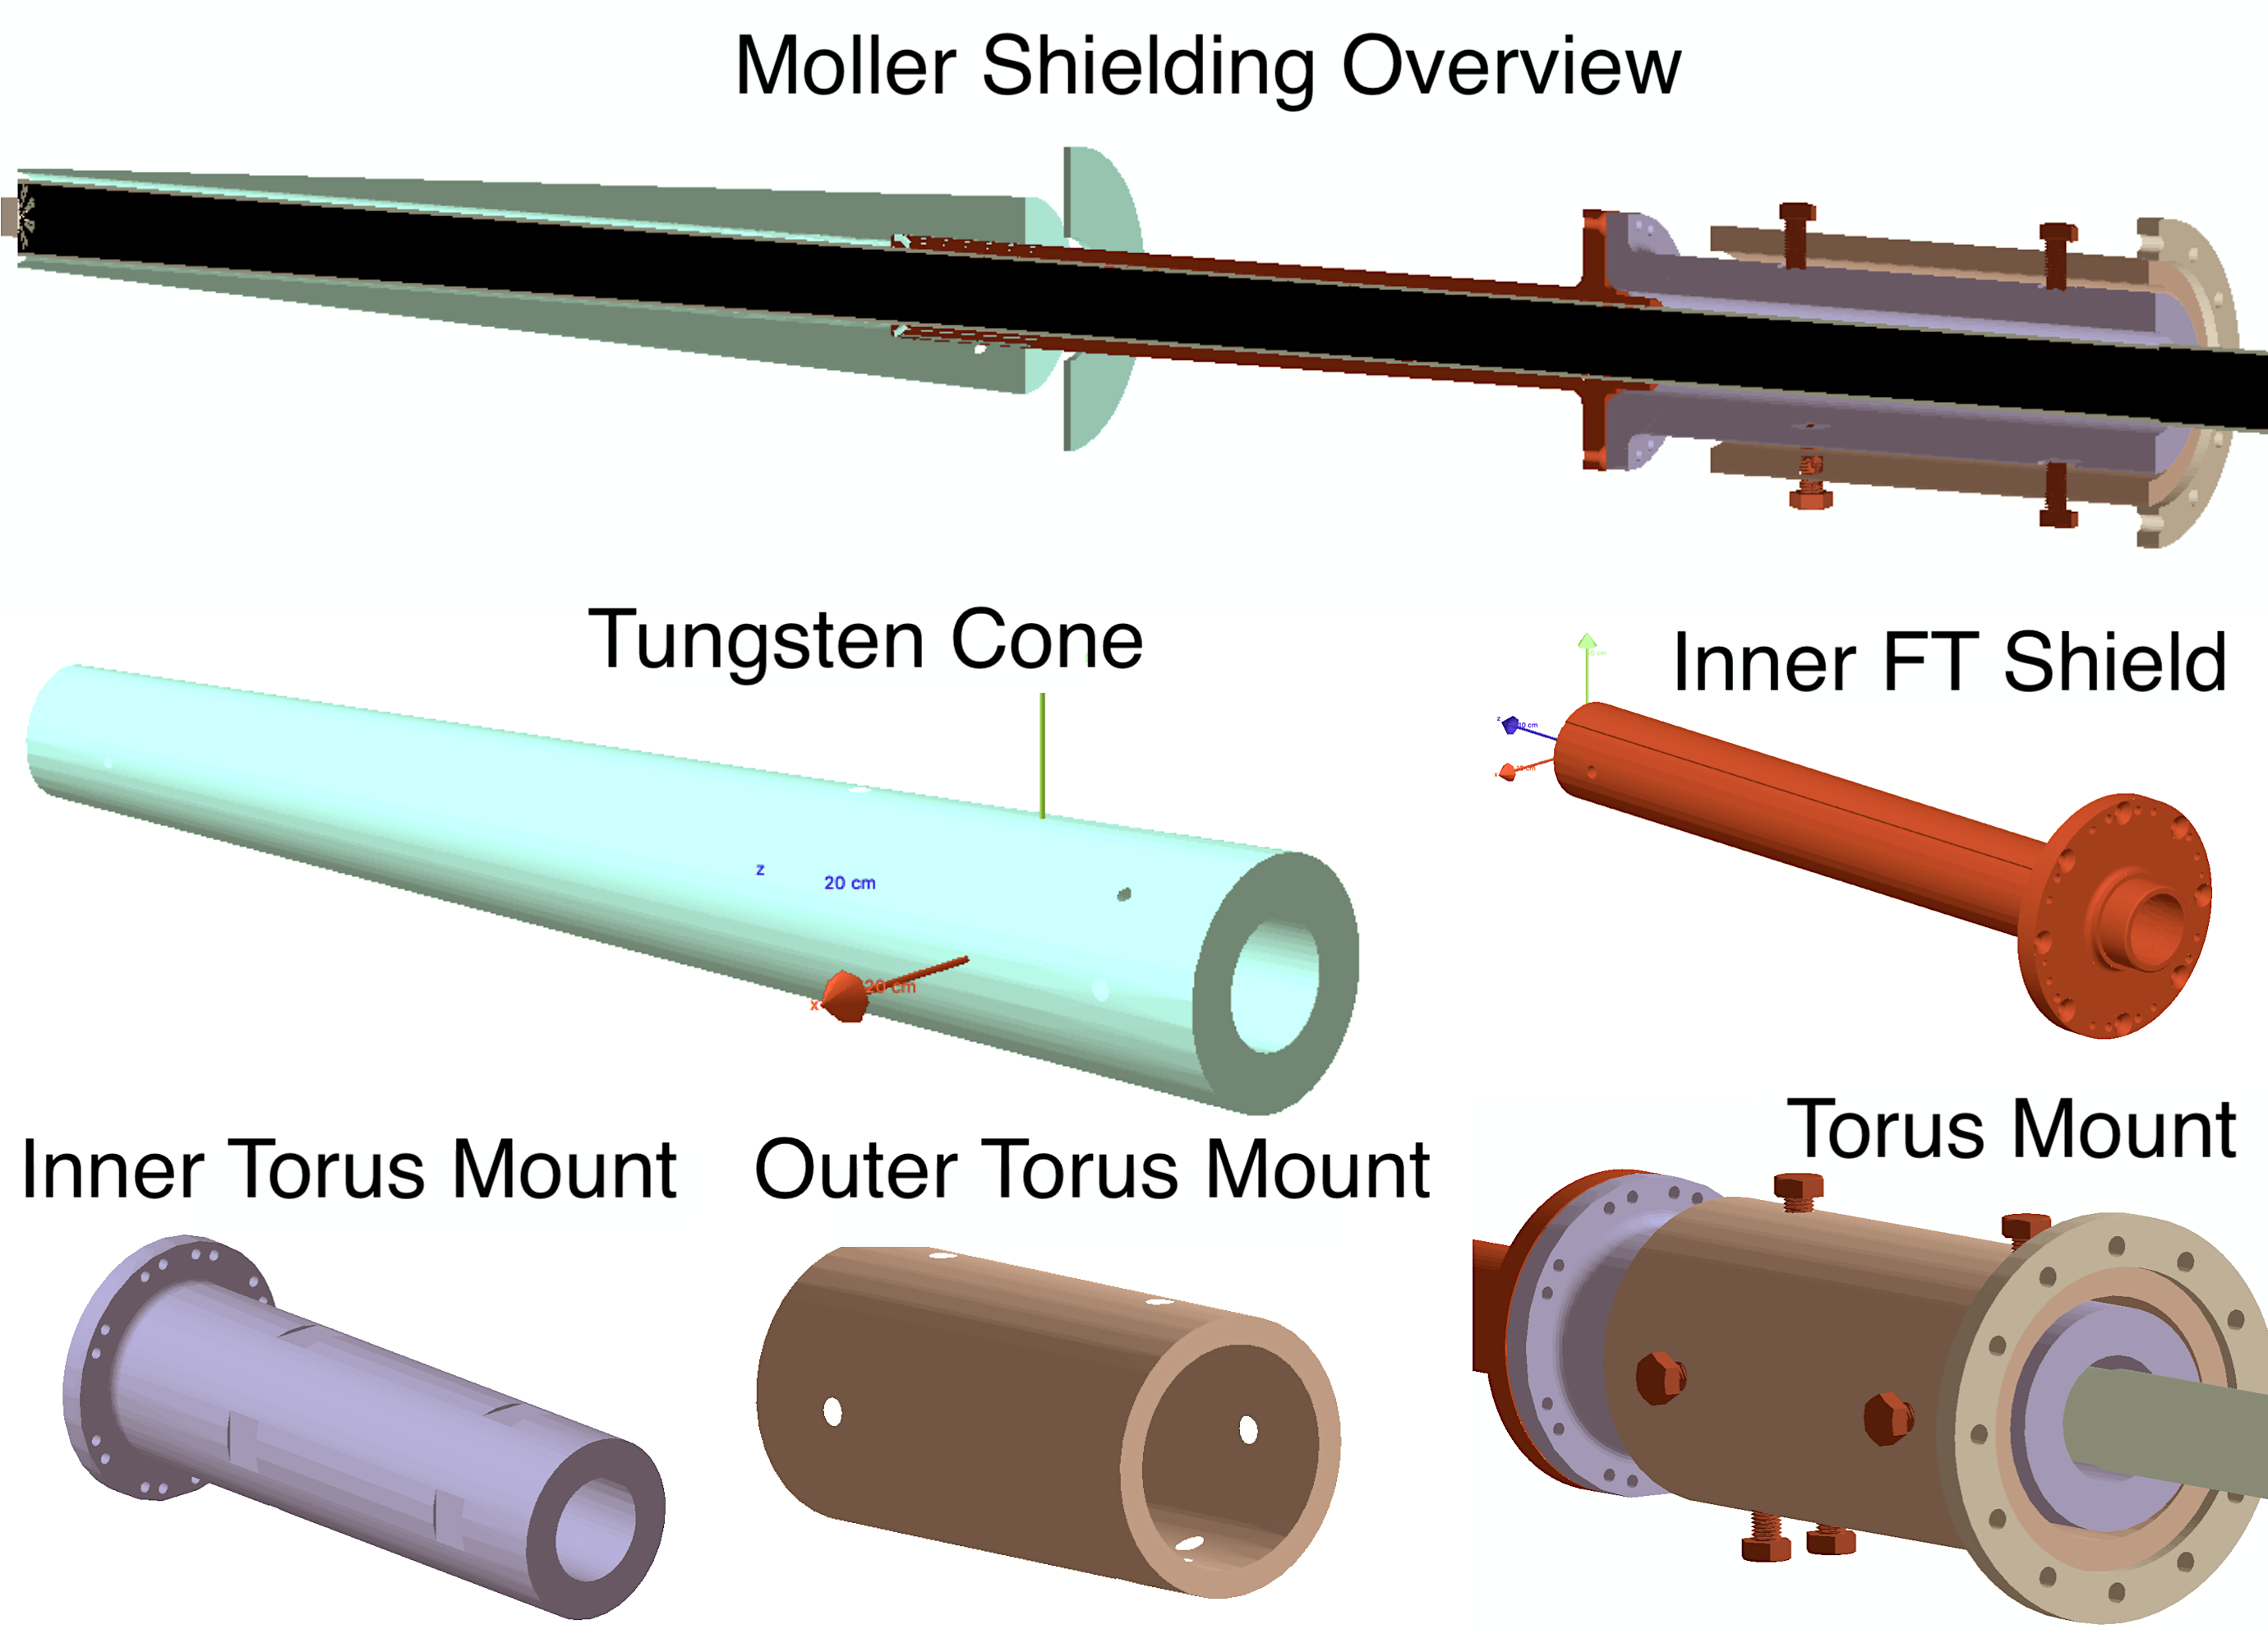
\includegraphics[width=0.98\columnwidth,keepaspectratio]{img/moellerShieldingFTOn.png}
	\caption{The moeller shielding for the FT On configuration. Top: section of the overall overview of the cone, FT support and torus mount.
		     Various individual components are shown: the tungsten cone, the inner FT shield, and the structure of the torus mount.}
	\label{fig:moellerShieldingFTOn}
\end{figure}

\begin{figure}
	\centering
	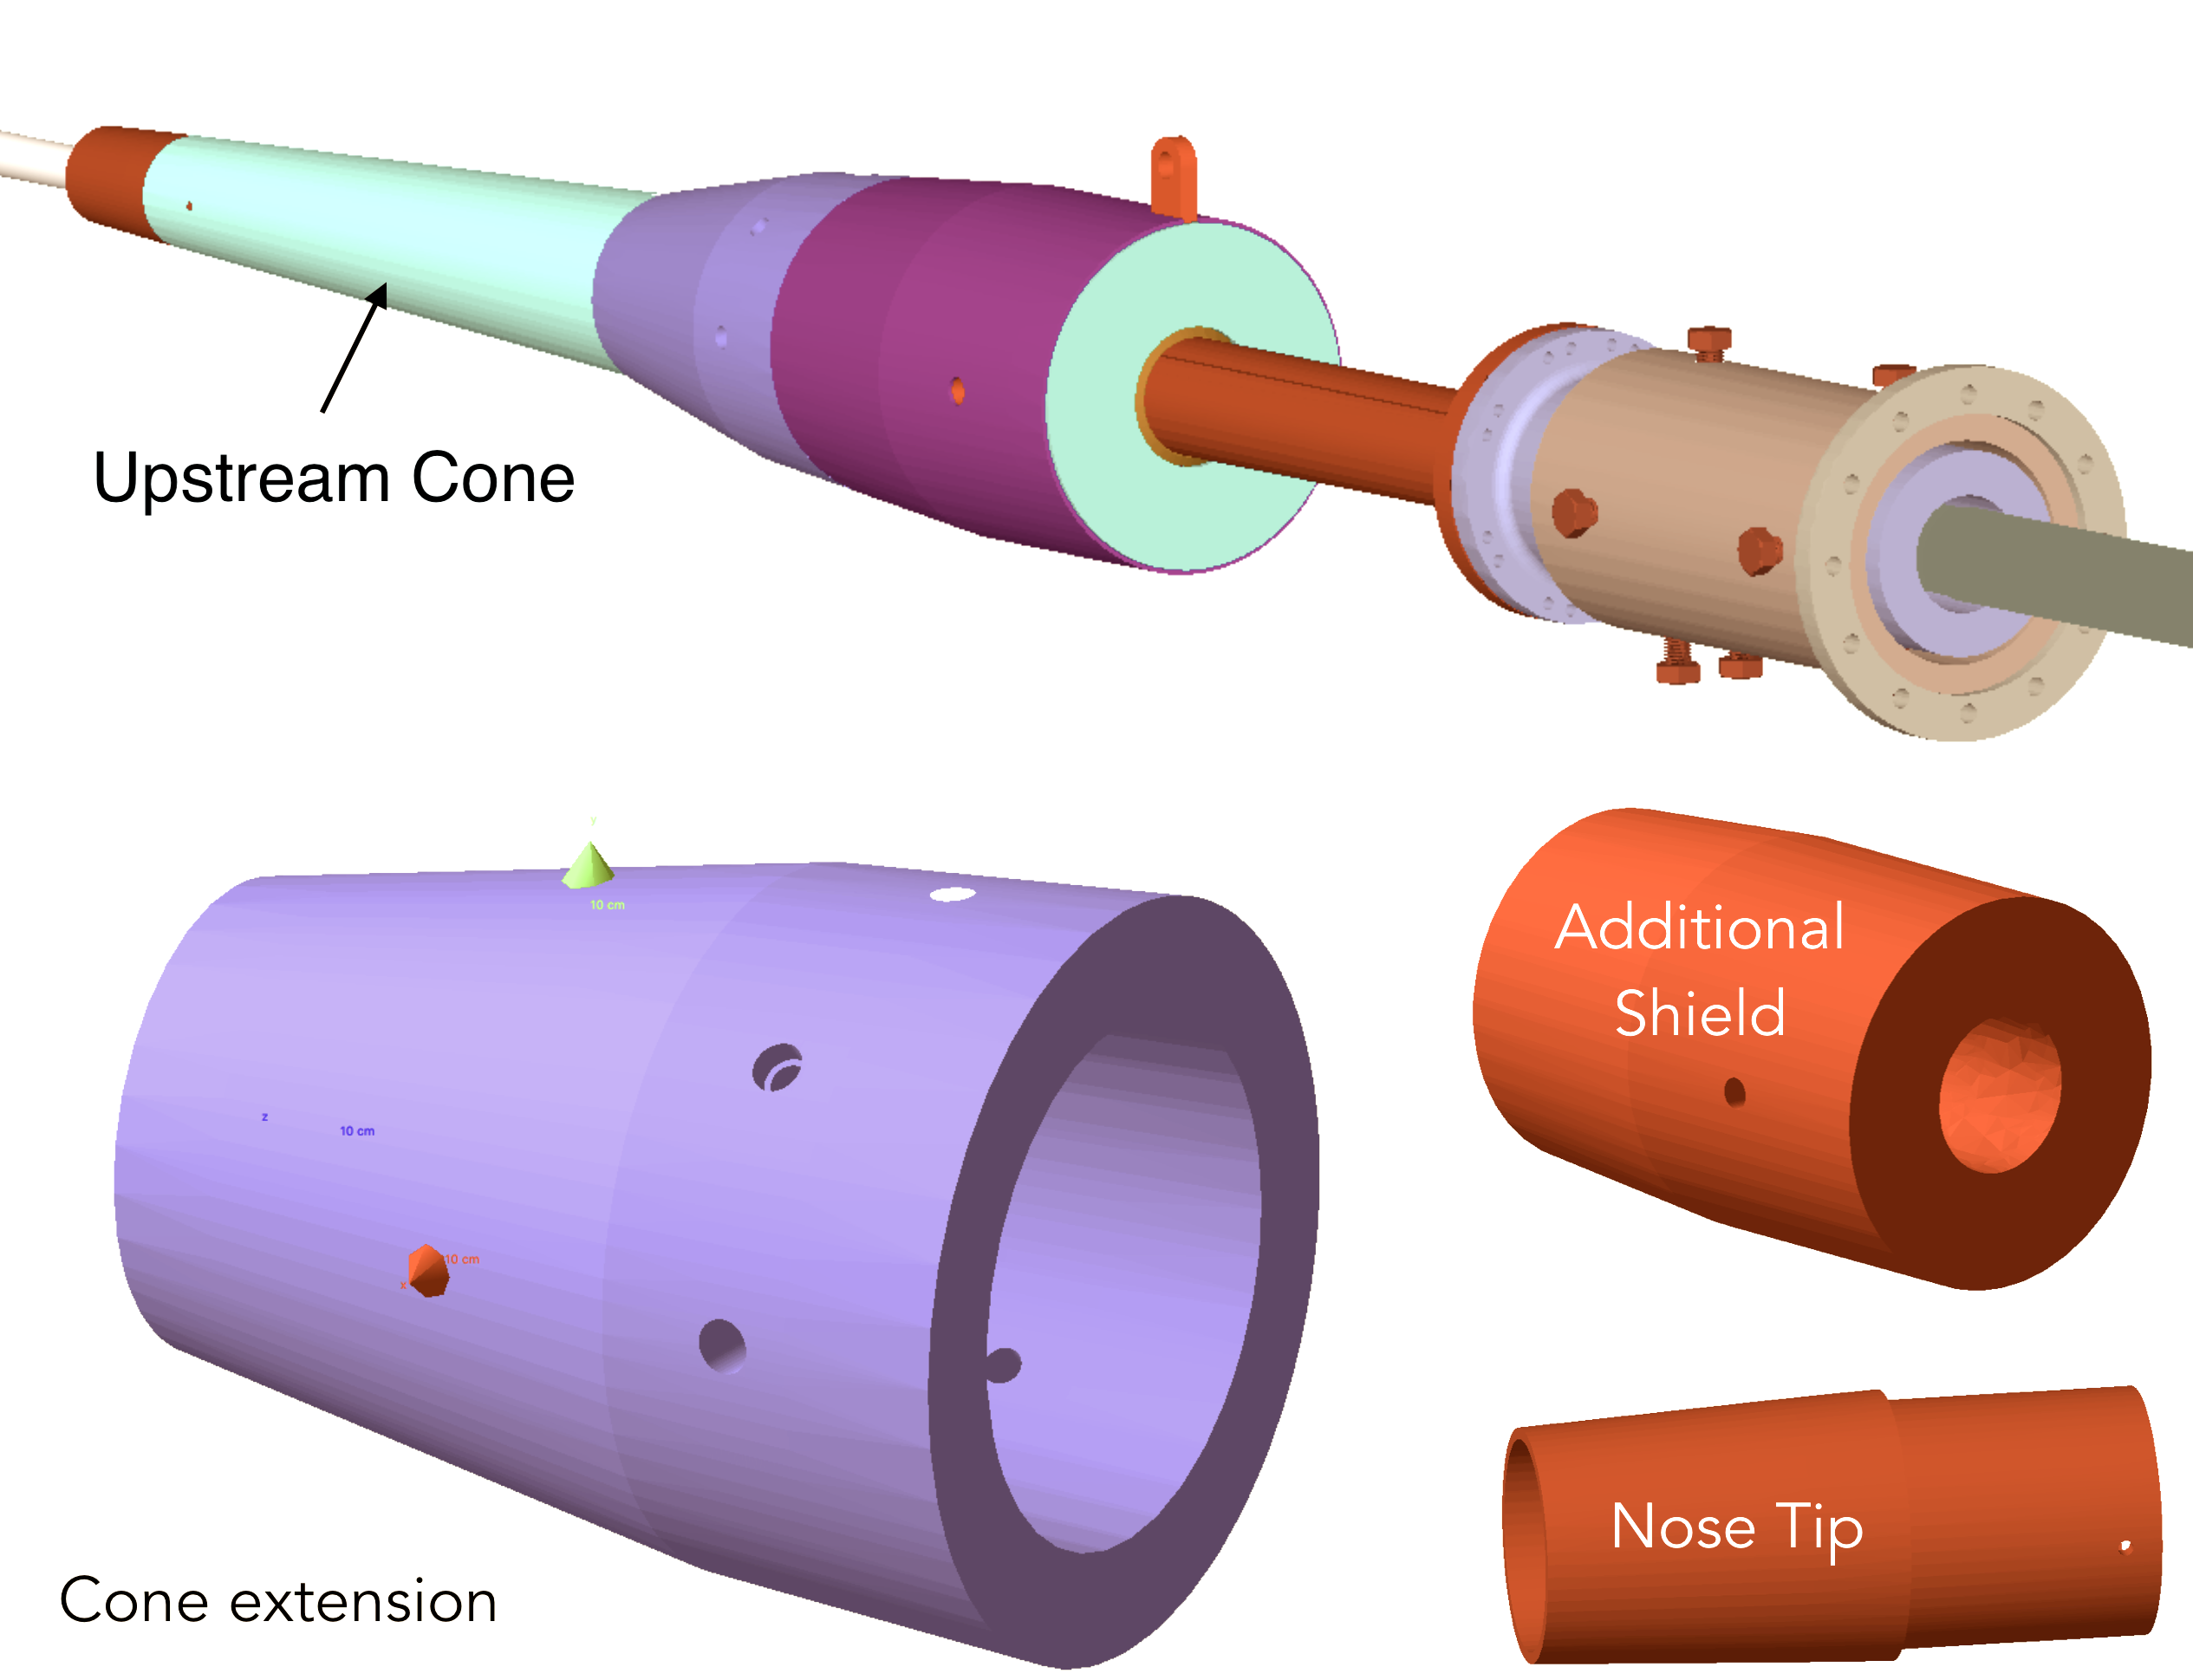
\includegraphics[width=0.98\columnwidth,keepaspectratio]{img/moellerShieldingFTOff.png}
   \caption{The moeller shielding for the FT Off configuration. Top: section of the overall overview of the cone, FT support and torus mount.
            the cone tip extension and the additional shielding that replace the FT tracker is also shown.}
	\label{fig:moellerShieldingFTOff}
\end{figure}



\begin{itemize}
	\item FT On and FT Off configurations:
	\begin{itemize}
		\item a Tungsten cone with increasing thickness.
		\item a tungsten pipe and flange inside the FT
		\item a structure to mount the FT and the shielding onto the torus frame, composed by:
		\begin{itemize}
			\item an inner stainless steel shield and flange
			\item an outer tungsten shield
			\item nine copper screw to adjust the alignment of the FT and shields upstream of the torus
		\end{itemize}
	\end{itemize}
	\item Only FT Off configuration:
	\begin{itemize}
	\item a Tungsten cone tip to extend the moeller shield cone
	\item additional lead structure to replace the FT tracker with shielding
	\end{itemize}

\end{itemize}




\subsection{Torus and downstream Shielding}
Additional shielding is placed around the vacuum pipe inside the torus hub in the form of tungsten bricks.
Downstream of the torus a shielding downstream of the torus in the form of a connecting tungsten nose and a long lead pipe.

These components are shown in \F{downstreamShielding}.

\begin{figure}
	\centering
	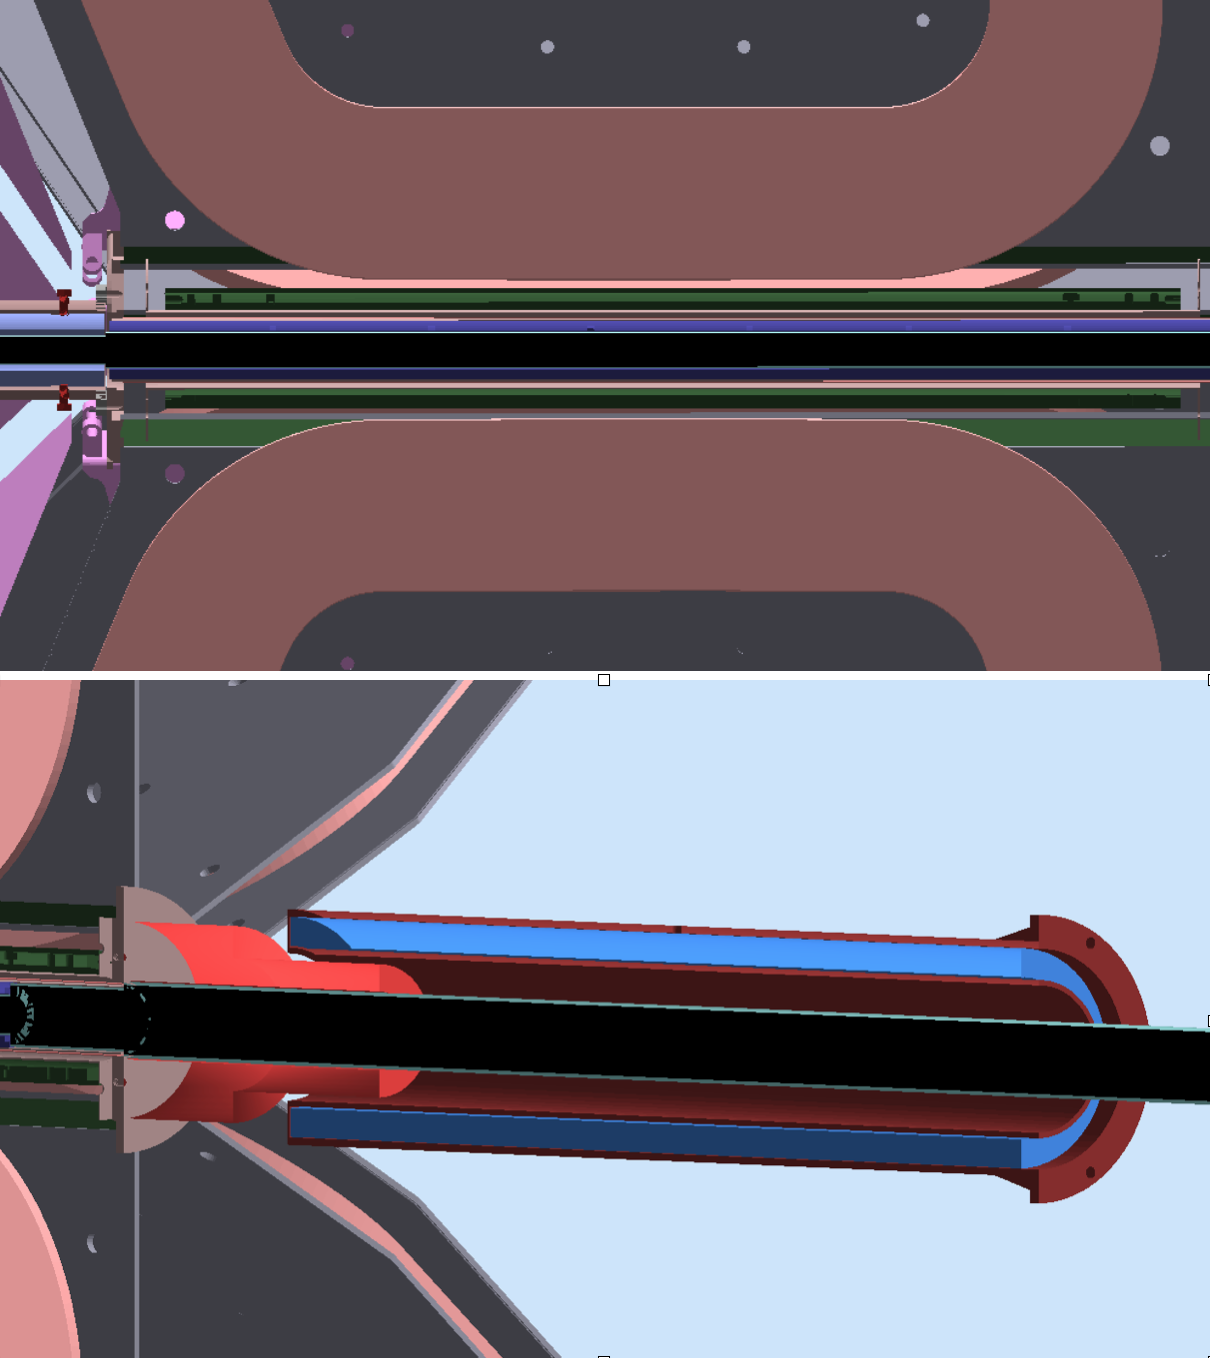
\includegraphics[width=0.98\columnwidth,keepaspectratio]{img/downstreamShielding.png}
   \caption{Torus and Downstream shielding.}
	\label{fig:downstreamShielding}
\end{figure}



\subsection{Geometry Source}

The beamline geometry is entirely imported from the engineering CAD model.

\subsubsection{Geometry Git Location}

The github location of the gemc geometry CAD volumes is \url{https://github.com/gemc/detectors/tree/master/clas12/cadBeamline}.
